\begin{abstract}
%% TODO(results): rewrite with final numbers from results/analysis.json
When a user asks an LLM search agent a question in Hindi or Telugu, the answer is less often right than when the same question is asked in English. Two different things can cause that, and they call for different fixes: the agent may search badly, or in a language where the evidence is not (the \emph{query-side gap}), or the evidence may simply not exist in that language (the \emph{evidence-side gap}). We separate them. We hold the question fixed with human-parallel Hindi/English and Telugu/English questions, hold the evidence fixed with a frozen two-language Wikipedia pool in which the gold passage is served in English only, in the Indic language only, or in both, log the script of every search query the agent writes under a free policy, and then force the query language (match, English, or both). The controlled conditional accuracies are weighted by the measured share of facts that the live Hindi and Telugu Wikipedias actually contain, which turns ``Hindi is worse'' into a decomposition of the real-world gap into a web term, an agent term, and a recoverable term. [RESULTS SENTENCES]
\end{abstract}

\section{Introduction}
\label{sec:intro}

Search agents, a language model that writes queries, reads what comes back, and answers, are now how hundreds of millions of people in India reach the web through chat products. When the question is in Hindi, Telugu, or Bengali rather than English, the answer is wrong more often. That much is established for browsing and deep-research agents across many languages \citep{a2505_15935,a2608_08775,a2606_15345,a2610_03574}. What is not established is \emph{why}, and the why decides the fix.

Two causes produce the same drop. The first is the agent. It may write a worse query in Hindi than in English, or it may write its query in a language where the evidence is not: an English query for a fact that only the Hindi Wikipedia records, or a Hindi query for a fact that only the English Wikipedia records. We call this the \textbf{query-side gap}. Prompting and training can fix it. The second is the web. Hindi Wikipedia has 2.4\% of the articles of English Wikipedia, Telugu 1.8\%, and Hindi is 0.2\% of Common Crawl pages. If the fact is not written in the user's language, no query will find it in that language, and the only remedies are cross-lingual search or writing the content. We call this the \textbf{evidence-side gap}. A residual remains when the right passage is in front of the model and it still answers worse in Hindi than in English; we call that the \textbf{integration gap}.

Nobody has separated these for a search agent. The closest study translates an English deep-research corpus into twelve languages and measures how much oracle retrieval recovers, but the question is always English, the agent's own query language is never observed or manipulated, and no Indic language is included \citep{a2606_15345}. A SIGIR 2026 study evaluates two web-search models on native Marathi queries and attributes failures to integration ``rather than missing sources'' by inspection, with one language and no manipulation \citep{kale2026marathiweb}. Single-shot retrieval work has named the confound, that an apparent preference for English evidence is partly an artefact of where gold evidence lives \citep{a2601_02956}, and has shown, with fixed context and no retrieval, that models prefer the query's language when a fact exists only in one Wikipedia edition, with Bengali the worst case \citep{a2610_00606}. English-only failure taxonomies split agent failures into ``never found'' and ``found but misused'' \citep{a2608_01913,a2608_05212}. None of these logs what language an agent searches in when a user asks in an Indic language, forces that language, and serves or withholds the evidence in each language on parallel questions.

We do that (Figure~\ref{fig:teaser}). Our instrument has three parts. \textbf{Parallel questions}: human-translated Hindi/English and Telugu/English question pairs from IndicGenBench XorQA-In \citep{a2404_16816} and natively parallel Hindi/English Wikipedia paragraphs from MLQA \citep{a1910_07475}, kept only when the Indic Wikipedia article verifiably states the answer, so that the evidence exists in both languages by construction. \textbf{A frozen two-language web}: the complete Hindi and Telugu Wikipedias and a sample of English Wikipedia from the same October 2026 snapshot, chunked and indexed, with the agent's single \texttt{search} tool served from the English-only pool, the Indic-only pool, or their union. \textbf{A query-language log and lever}: under a free policy we record the script of every query the agent writes; under three forced policies the agent must query in the question's language, in English, or in both. A closed-book arm measures what the model already knew, and an oracle arm with the gold passage in the prompt measures the integration gap. Because dense multilingual retrieval is cross-lingual and lexical retrieval is not, we run the grid under both a bge-m3 dense retriever and BM25: whose language the search engine speaks is itself part of the query-side gap.

The controlled grid gives conditional accuracies. To turn them into a statement about the real web we measure coverage: for 539 XorQA questions per language, whether the Hindi or Telugu Wikipedia article linked to the English source article states the answer (string match, two independent LLM reads of the article, and a manual audit). The decomposition
\begin{equation}
\mathrm{Acc}_L \;=\; \mathrm{Cov}_L \cdot \mathrm{Acc}(L \mid \text{evidence in } L) \;+\; (1-\mathrm{Cov}_L)\cdot \mathrm{Acc}(L \mid \text{evidence only in English})
\label{eq:decomp}
\end{equation}
then says how many points of the Indic user's deficit are the web's, how many are the agent's, and how many a different query policy recovers.

\paragraph{Findings.}
%% TODO(results): five numbered findings with numbers, CIs, BH status, section refs
\begin{enumerate}
\item \textbf{[D1 query-language drift]} \ldots
\item \textbf{[D2 query-side gap and recovery]} \ldots
\item \textbf{[D3 policy $\times$ evidence interaction]} \ldots
\item \textbf{[D4 coverage and the decomposition]} \ldots
\item \textbf{[D5/D6 retriever and integration]} \ldots
\end{enumerate}

\begin{figure}[t]
\centering
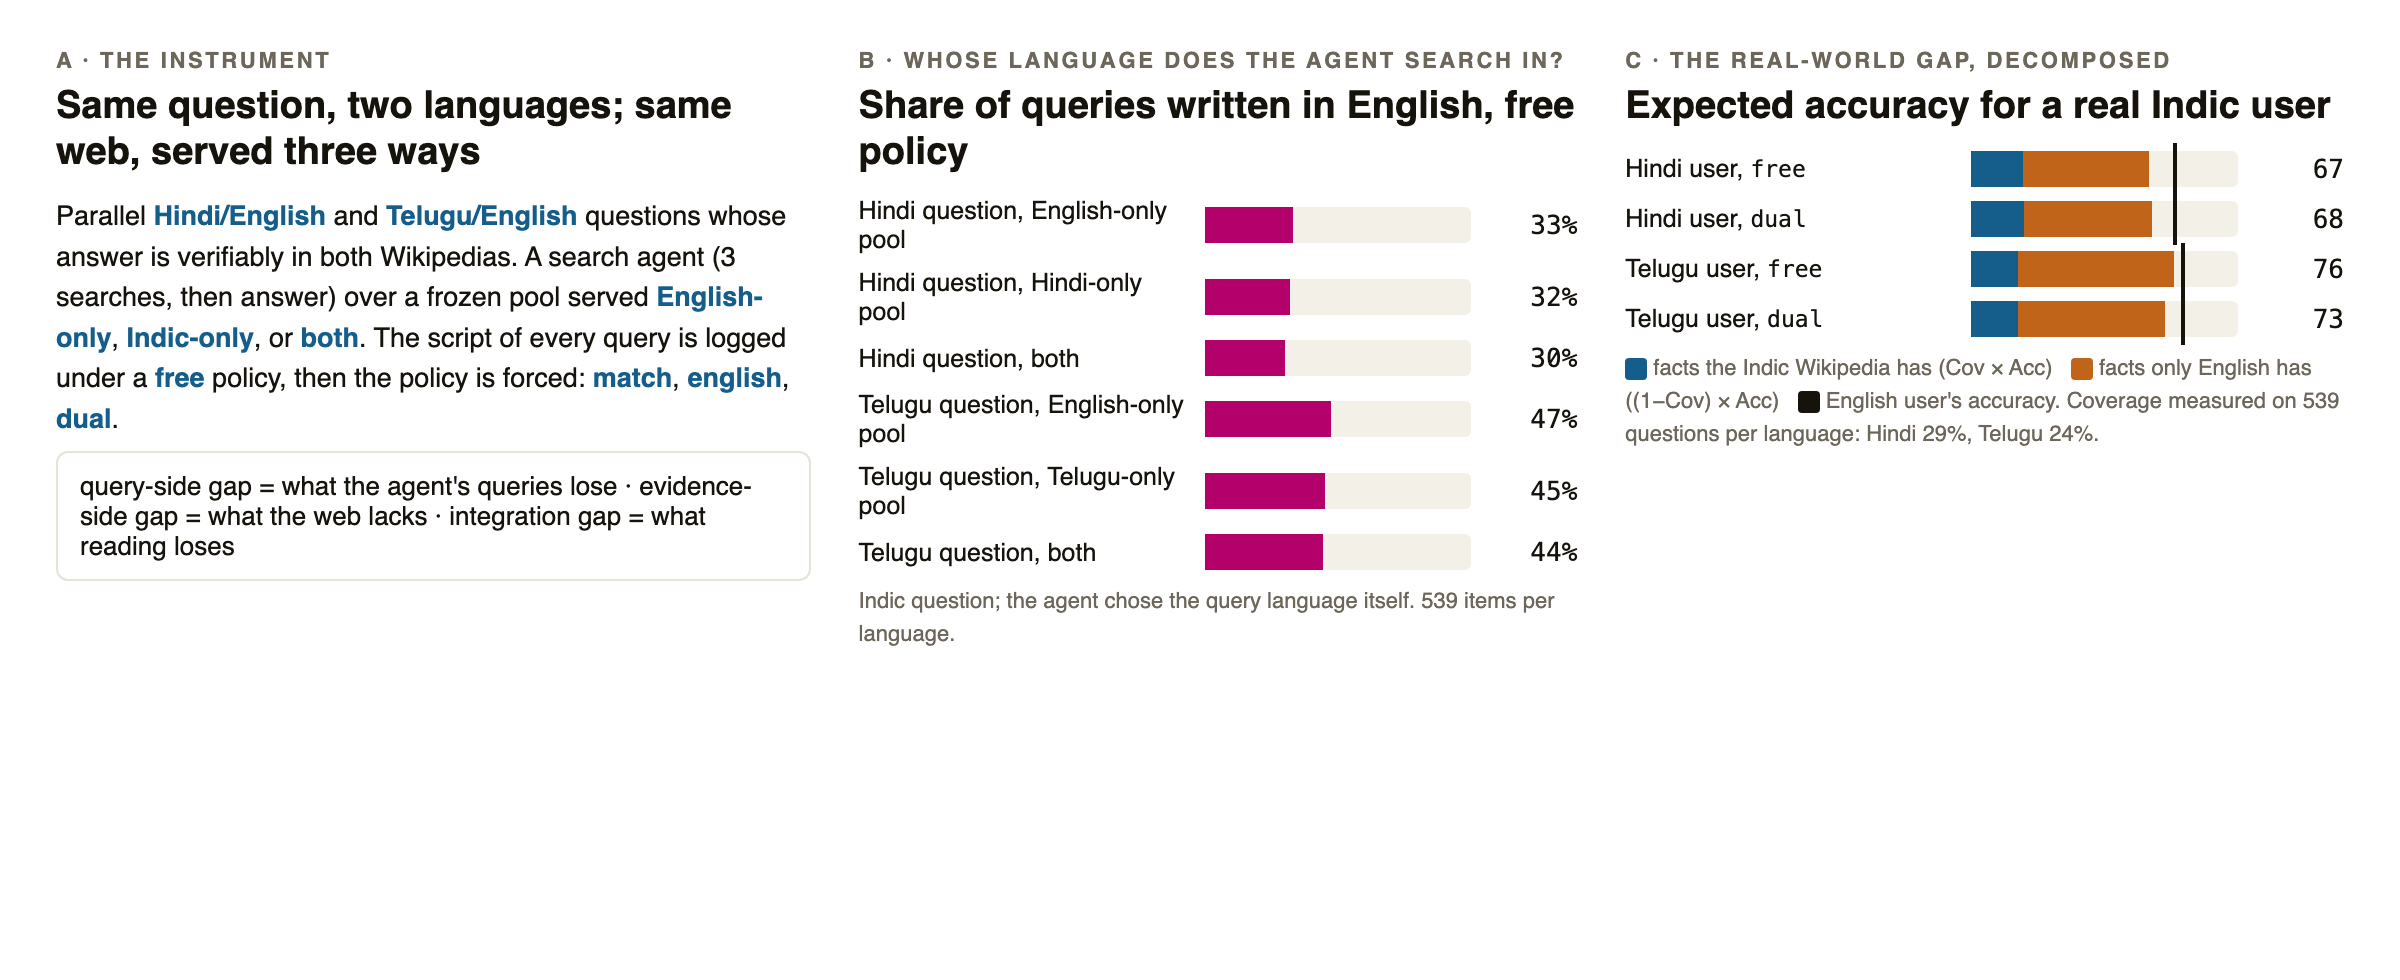
\includegraphics[width=\textwidth]{assets/fig1_teaser.png}
\caption{%% TODO(results)
Study design and headline numbers. Parallel Hindi/Telugu and English questions; a frozen two-language Wikipedia pool served English-only, Indic-only, or both; the agent's query script logged under a free policy and then forced; coverage measured on the live Indic Wikipedias; the decomposition of the real-world gap into web, agent, and recoverable terms.}
\label{fig:teaser}
\end{figure}

\paragraph{Pre-registration.} Six directional predictions (D1--D6) were written into the project log before any grid call, with the falsification conditions. [TODO: which held, which failed.] Failures are reported in the abstract and in Section~\ref{sec:results}.

\paragraph{Responsible framing.} Only public Wikipedia text (CC BY-SA) and public benchmark questions are used; the pools regenerate from the public snapshot and our scripts. Models are queried through their public APIs or an open-weight checkpoint on our own GPU. No deployed search product is probed.

\section{What was known and what is new}
\label{sec:known}

We want to be plain about what is already established. That LLM agents do worse on non-English tasks is known: GAIA in eleven languages scores 47.4\% in English against 35.8\% elsewhere, Hindi included \citep{a2505_15935}; GAIA2 in ten languages finds Hindi the weakest at every model size \citep{a2608_08775}; natively authored browsing questions in thirteen languages differ by language \citep{a2610_03574}. That retrievers and generators prefer English and query-language passages is known \citep{a2502_11175,a2604_20199,a2509_13930}. That the apparent English preference is partly an artefact of where gold evidence lives is known for single-shot RAG \citep{a2601_02956}. That models write tool arguments in the wrong language is known, Hindi included \citep{a2601_05366}. That parametric knowledge of India-centric facts is weaker in Indic scripts is known \citep{a2504_20022,a2605_29637,a2504_10356,a2610_00606}. That agent failures split into retrieval and utilisation is known for English \citep{a2608_01913,a2608_05212,a2609_08094}.

\begin{table}[h]
\small
\centering
\begin{tabular}{p{3.6cm}p{9.6cm}}
\toprule
\textbf{Closest neighbour} & \textbf{What it established / what it does not cover} \\
\midrule
XBCP \citep{a2606_15345} & Deep-research agents on BrowseComp-Plus with the corpus translated into 12 languages; oracle decomposition into retrieval vs integration. Question always English; query language never logged or forced; no Indic language; translated rather than native evidence. \\
MarathiWeb \citep{kale2026marathiweb} & Two web-search LLMs on native Marathi queries; failures attributed to integration by inspection. One language; evidence availability observed, not manipulated; no parallel English arm. \\
MAST Indic track \citep{mast2026} & Nine Indic query languages over the English BrowseComp-Plus corpus. English-only corpus, so the evidence-side gap is zero by construction; a systems shared task. \\
DELTA \citep{a2601_02956} & Names the gold-availability prior and regresses it out of single-shot RAG. No agent, no Indic, statistical rather than experimental control. \\
Where's Waldo \citep{a2610_00606} & Query-language preference with fixed paired context when a fact exists in one edition only; Bengali worst. No retrieval, no agent, no search-query language. \\
Diagnosing search failures \citep{a2608_01913} & Retrieval gap vs utilisation gap with oracle evidence. English only; the retrieval gap is not split into query formulation vs corpus coverage. \\
Cross-Lingual Cost \citep{a2507_07543}; XRAG \citep{a2505_10089}; tRAG/CrossRAG \citep{a2504_03616}; CORAL \citep{a2604_25676} & Query-language vs document-language effects in RAG; one controlled Google ablation; an agent that picks the corpus language. Non-agentic or end-accuracy only; no Indic; no decomposition. \\
\bottomrule
\end{tabular}
\caption{Novelty delineation. Full related work in Section~\ref{sec:related}.}
\label{tab:delineation}
\end{table}

What is new here is (i) the agent's search-query language as a measured mediator and then a manipulated factor, (ii) parallel Indic/English questions over a frozen evidence pool in which the language of the gold evidence is served or withheld, (iii) the retriever (cross-lingual dense vs monolingual lexical) as a factor in the query-side gap, and (iv) a coverage term measured on the live Indic Wikipedias that weights the controlled accuracies into a real-world decomposition.

\section{Method}
\label{sec:method}

\subsection{Questions}
\label{sec:questions}
%% numbers fixed by corpus/FROZEN.json
\textbf{XorQA-In} \citep{a2404_16816} provides 539 test questions per language, human-translated from the English TyDi XOR questions \citep{a2010_11856}, each with the English Wikipedia paragraph that answers it and the English answer. For each item we located the Hindi or Telugu counterpart of the English source article through Wikidata sitelinks (916 of 918 titles resolved) in the same snapshot and checked whether that article states the answer: by answer-string match in either script, then by two independent LLM reads of the full article (gemini-2.5-flash-lite, then gemini-3.6-flash) that had to quote a sentence found verbatim in the article, with a 50-item manual audit (Appendix~\ref{app:coverage}). An item enters the controlled grid only when both reads agree and the quoted or matched sentence exists: 157 Hindi and 127 Telugu items. The Telugu translated answers in the release are unusable for 237 items (the string ``{\telu అని}'', ``that''), so Telugu answers are scored against the English gold and by an LLM judge. \textbf{MLQA} \citep{a1910_07475} provides 4{,}918 Hindi questions whose English counterparts share ids and whose Hindi and English paragraphs are naturally parallel Wikipedia text; many MLQA questions presuppose their paragraph (``What did Keane often request?''), so we kept only questions an LLM filter judged self-contained (176 of 450 checked) and sampled 130. Both gold paragraphs are injected into the pools. \textbf{TyDi XOR} Telugu validation questions (120 sampled from 291 answerable), natively written rather than translated, form a robustness subset for the translation-artefact concern \citep{a2604_24929}; they have no English twin and are run in Indic-question cells only. Every item carries its English and Indic gold answers; the full bank with the coverage flags is frozen with SHA-256 hashes.

\subsection{The frozen two-language web}
\label{sec:pool}
All pools come from one snapshot, \texttt{wikipedia-monthly} 20261001 \citep{wikipediamonthly2026}: the complete Hindi Wikipedia (169{,}949 articles, 353{,}075 chunks), the complete Telugu Wikipedia (145{,}514 articles, 518{,}524 chunks), and a 1.8\% sample of English Wikipedia (129{,}646 articles, 1{,}058{,}175 chunks) to which we add the full English article behind every item (681 articles, 7{,}310 chunks) and 666 deduplicated gold paragraphs. Articles are split into chunks of about 900 characters with the title prefixed. The agent's one tool, \texttt{search(query)}, returns the top five chunks from the pool being served: English-only, Indic-only, or their union. We run two retrievers. BM25 \citep{robertson2009bm25,a2407_03618} over Unicode word tokens with no stemming is the lexical instrument; bge-m3 dense embeddings \citep{a2402_03216} with exact inner-product search are the semantic one. A sanity check with the question itself as the query put the gold chunk in the top five for 50\% of English questions under BM25 but only 8\% of Hindi and 7\% of Telugu ones (transliteration variants such as {\deva ओरेगन}/{\deva ऑरेगॉन} and Telugu case suffixes defeat exact tokens); bge-m3 gave 70\% for both Indic languages and retrieved Hindi gold for English queries 68\% of the time. The dense retriever is therefore the main-grid instrument and BM25 the comparison; the difference between them is part of what we measure.

\subsection{The agent and the policies}
\label{sec:agent}
A fixed ReAct loop \citep{a2210_03629} over native tool calling: a system prompt, the question, at most three \texttt{search} calls, then a short final answer in the question's language; temperature 0; minimal reasoning effort. The only text that differs between policy cells is one sentence: none (\textbf{free}), ``write every query in [the question's language]'' (\textbf{match}), ``write every query in English'' (\textbf{english}), or ``at every step search once in each language'' (\textbf{dual}). For every search call we log the query, its dominant Unicode script (Devanagari, Telugu, Latin, or mixed), the languages of the five hits, and whether a gold chunk was among them. Verbatim prompts are in Appendix~\ref{app:prompts}.

\subsection{Factors, arms, and models}
\label{sec:factors}
Question language $Q\in\{\text{en}, L\}$; policy $P\in\{\text{free, match, english, dual}\}$; evidence pool $E\in\{\text{en-only}, L\text{-only}, \text{both}\}$. The core grid is $Q{=}L\times 4P\times 3E$ plus $Q{=}\text{en}\times\{\text{free, match}\}\times 3E$ plus $Q{=}\text{en}\times\text{dual}\times L$-only: 19 cells, every factorial item, both languages, under the dense retriever; the same 19 cells under BM25 for the cheapest model and the eight headline cells for the others. Arms: \textbf{closed-book} (no tool, $Q\in\{\text{en},L\}$) for parametric leakage; \textbf{oracle} (gold passage in the prompt, $Q\in\{\text{en},L\}$) for the integration gap; \textbf{none} (the pool with the item's gold removed, 50 items per language) for the abstention floor; a \textbf{repeat battery} (30 items $\times$ 5 identical runs) for the noise floor; and the \textbf{native-Telugu} subset. Models: gemini-2.5-flash-lite (full grid and all arms), gemini-3.1-flash-lite (120 items per language), gemini-3.6-flash (headline cells, 60 items per language), all through OpenRouter, and Qwen3-30B-A3B-Instruct-2507 served with vLLM on a rented GPU as the open-weight family. Other closed families were blocked by a workspace guardrail on the API account at the time of the study (Section~\ref{sec:limits}).

\subsection{Scoring and statistics}
\label{sec:stats}
An answer is correct if it matches a gold alias in either script after normalisation (digit systems unified, 40-character containment slack), otherwise a judge model not in the grid (gemini-2.5-flash) labels it CORRECT, WRONG, or ABSTAIN from the English and original question and all gold aliases; 40 judged items are hand-audited (Appendix~\ref{app:audit}). The unit is the item. Every contrast is a paired within-item difference with a sign-flip permutation test (20{,}000 draws) and an item-bootstrap 95\% interval (10{,}000 draws); the policy $\times$ evidence interaction is tested by label permutation (5{,}000); all reported $p$-values form one Benjamini--Hochberg family \citep{benjamini1995bh} and only survivors are set in bold. Every number traces to one analysis script.

\section{Results}
\label{sec:results}

Table~\ref{tab:main} lists every paired contrast with its interval, permutation $p$-value and Benjamini--Hochberg status; Appendix~\ref{app:cells} lists every cell. All numbers are accuracies in percentage points on the factorial items (287 Hindi, 127 Telugu). The repeat battery (30 items $\times$ 5 identical runs, Indic question, free policy, both pools) changed the verdict on 1 of 30 Hindi items and 0 of 30 Telugu items, so cell-level differences below about two points are within the noise floor and are not interpreted.

\subsection{In what language do agents search?}
\label{sec:results-drift}

Under the free policy, with the question in Hindi, Gemini 2.5 Flash-Lite writes 30--33\% of its search queries in English, Gemini 3.1 Flash-Lite 31--38\%, Gemini 3.6 Flash 45--57\%, and Qwen3-30B-A3B 18--19\% (Figure~\ref{fig:fig2}). With the question in Telugu every model searches in English more often: 44--48\% for the three Gemini models and 43--46\% for Qwen. Mixed-script queries are rare (0--3\%, 15\% for Gemini 3.6 Flash on the English-only pool). The shares barely move with the pool that is served: the agents do not notice that an English-only pool returned no Hindi text and switch. Pre-registered direction D1 predicted a majority of English queries; that holds for one model and one pool (Gemini 3.6 Flash, Hindi question, English-only pool, 57\%) and fails elsewhere. The second half of D1, more English for Telugu than for Hindi, holds for every model except Gemini 3.6 Flash, where the two are equal.

\subsection{The query-side gap and how much a policy recovers}
\label{sec:results-qg}

With evidence present in both languages and the dense retriever, the Hindi question costs Gemini 2.5 Flash-Lite 9.4 points against the English question (66.2 vs 75.9, interval 4.5 to 14.3, survives correction) and Qwen3-30B-A3B 9.1 points (65.5 vs 74.6, survives). The two stronger Gemini models show no measurable gap: 3.0 points for 3.1 Flash-Lite (interval $-2.0$ to $8.0$) and 2.0 points for 3.6 Flash (interval $-4.0$ to $8.0$). For Telugu the gaps are 4.7, 1.0, $-6.0$ and 2.4 points, none significant. The gap is a property of the cheaper models, not of the languages.

Where the gap exists, forcing the query language does not close it. On Gemini 2.5 Flash-Lite, Hindi question, both pools: matched-language queries change accuracy by $+0.7$ points, dual-language queries by $+1.8$, English-only queries by $+4.5$ (interval $0.0$ to $9.1$, $p=0.07$, not surviving correction). Gold passages are already in the top five for 79\% of free-policy episodes and 87\% of dual-policy episodes, so there was little retrieval to recover. On Qwen the dual policy recovers 4.5 of the 9.1 points ($p=0.035$, not surviving). D2 (a query-side gap that dual queries halve) is therefore supported in direction for Qwen and not for Gemini; the measured query-side gap under cross-lingual retrieval is at most a few points.

Under BM25 the same model and items tell a different story (Figure~\ref{fig:fig5}, Table~\ref{tab:main}, rows marked BM25). The Hindi question now costs 18.9 points (50.3 vs 71.4, survives), the Telugu question 11.0 points, and the Indic question with the lexical retriever scores 15.7 points (Hindi) and 21.3 points (Telugu) below the same question with the dense retriever (both survive). Here the policy matters: dual queries recover 9.3 of the 18.9 Hindi points (survives), and the English-only policy on the English-only pool reaches 62.7 against 43.4 under the free policy. Gold passages reach the top five in 40\% of free-policy episodes under BM25 against 79\% under dense retrieval, and the agent abstains in 23--39\% of BM25 episodes against 6--8\% with dense retrieval. The query-side gap is large when the search engine is monolingual and nearly absent when it is cross-lingual.

\subsection{Policy \texorpdfstring{$\times$}{x} evidence: when searching in English helps and when it hurts}
\label{sec:results-interaction}

Pre-registered direction D3 said that forcing English queries helps when the evidence is English-only and hurts when it is Indic-only. On Gemini 2.5 Flash-Lite with Hindi questions this is what happens: English queries beat matched-language queries by 6.3 points on the English-only pool (survives) and lose 4.9 points on the Indic-only pool ($p=0.10$); the interaction is 11.2 points (interval 4.2 to 18.2, survives). The same model with Telugu questions shows no interaction (1.6 points), and neither does Gemini 3.1 Flash-Lite (3.0 and 2.0 points). The sign-flip predicted by the disagreement between query-translation studies \citep{a2507_07543,a2504_03616} is real, but only for the model and language where lexical cues still matter to a dense retriever: Hindi queries on English text retrieve the gold chunk 66\% of the time and English queries on Hindi text 68\%, so the policy mostly decides which pool the agent can read.

\subsection{Coverage and the decomposition of the real-world gap}
\label{sec:results-decomp}

Of the 539 XorQA questions per language, the linked Hindi Wikipedia article exists for 67.5\% and verifiably states the answer for 29.1\% (interval 25.2 to 33.0); for Telugu the article exists for 52.5\% and states the answer for 23.6\% (20.0 to 27.1). D4's first clause holds (both below one half, Hindi above Telugu). The manual audit of 50 items (Appendix~\ref{app:coverage}) found the first LLM read too generous, which is why a second read was required; the coverage estimates are the two-read figures.

Table~\ref{tab:decomp} and Figure~\ref{fig:fig4} put the coverage into Eq.~\ref{eq:decomp}. With the dense retriever the evidence-side term vanishes: for every model the Indic question on the English-only pool scores within two points of the same question on both pools (Table~\ref{tab:main}, evidence-side rows), because the retriever finds the English gold for a Hindi or Telugu query. The expected accuracy of a Hindi user is therefore 66.7 (Gemini 2.5 Flash-Lite), 76.4 (3.1 Flash-Lite) and 74.0 (3.6 Flash) against 75.8, 77.0 and 76.0 for an English user; the whole remaining gap is the agent's reading, not the web. D4's second clause, that the coverage term would exceed the agent term for Telugu, fails under cross-lingual retrieval. Under BM25 it is the other way round: the Hindi user of Gemini 2.5 Flash-Lite gets 45.4 against 71.4 for the English user, the Telugu user 49.9 against 66.9, and most of that loss is the 71\% of facts that only English Wikipedia holds, which a Hindi or Telugu query cannot reach lexically. Telling the agent to search in English lifts the Hindi user to 62.9 and the Telugu user to 67.1. So the advice to a product team depends on the engine: with lexical search, translate the query; with cross-lingual dense search, the query language is not the problem.

\subsection{The retriever, the oracle, and the open-weight model}
\label{sec:results-retriever}

The symmetric monolingual check (English question on the English-only pool against the Indic question on the Indic-only pool, matched queries) is 10.1 points for Hindi and 12.6 for Telugu under dense retrieval and 35.3 and 31.0 under BM25 (all survive), and with the gold passage in the prompt it is 6.3 points for both languages (Hindi survives; Telugu $p=0.10$): D5 holds. With the passage given, Gemini 2.5 Flash-Lite answers the Hindi question from the English passage 80.5\% of the time and from the Hindi passage 72.8\%; the model reads English evidence better than Hindi evidence even for a Hindi question. The two stronger Gemini models read as well in Hindi as in English (integration gaps of $-2.0$ and $-2.0$ points), so D6 holds for them and fails by 1.3 points for Gemini 2.5 Flash-Lite. Closed-book, the models already know many of these facts (57.8\% to 70.0\% for Hindi questions, 64.6\% to 84.0\% for Telugu), with closed-book gaps of 2--4 points; 77\% (Hindi) and 76\% (Telugu) of correct agent answers on Gemini 2.5 Flash-Lite had a gold chunk in their trajectory. On the pre-specified needs-search subset (97 Hindi items Gemini 2.5 Flash-Lite got wrong closed-book in both languages) the Hindi gap is 12.5 points ($p=0.02$) and dual queries recover 7.4 ($p=0.15$). With the gold evidence hidden from the pool the Hindi agent still scores 55.1\%, close to its closed-book 57.8\%, and abstains in 10\% of episodes.

The natively written Telugu questions (TyDi XOR, 120 items, Appendix~\ref{app:cells}) are harder than the translated ones (60.0\% against 74.8\% on the both-pools cell, different items), but the agent behaves the same way on them: 44\% English queries under the free policy against 44--47\% on the translated set, and no gain from dual queries. The translation of the questions does not drive the query-language behaviour.

\paragraph{Qwen3-30B-A3B.} %% TODO(qwen): finalise once the bm25 head, closed and oracle arms are in
The open-weight model behaves like the cheaper Gemini: a 9.1-point Hindi gap (survives), a 2.4-point Telugu gap, 18\% English queries for Hindi questions, 4.5 points recovered by dual queries, and no loss from the Indic-only pool. [QWEN BM25, closed-book and oracle numbers.]

\begin{figure}[t]\centering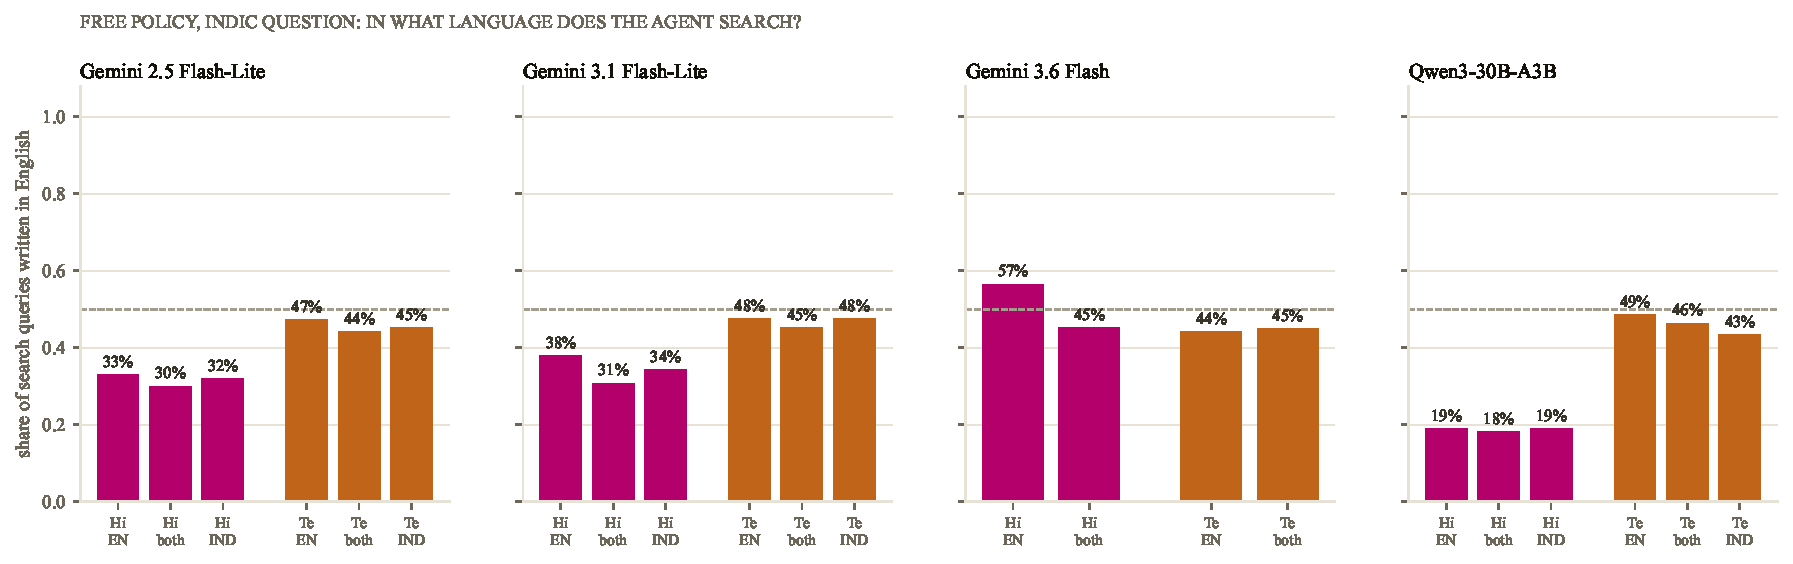
\includegraphics[width=\textwidth]{assets/fig2_query_language.pdf}
\caption{Share of search queries written in Latin script when the question is in Hindi (magenta) or Telugu (orange), free policy, by served pool (EN = English-only, IND = Indic-only). Dashed line: one half.}\label{fig:fig2}\end{figure}
\begin{figure}[t]\centering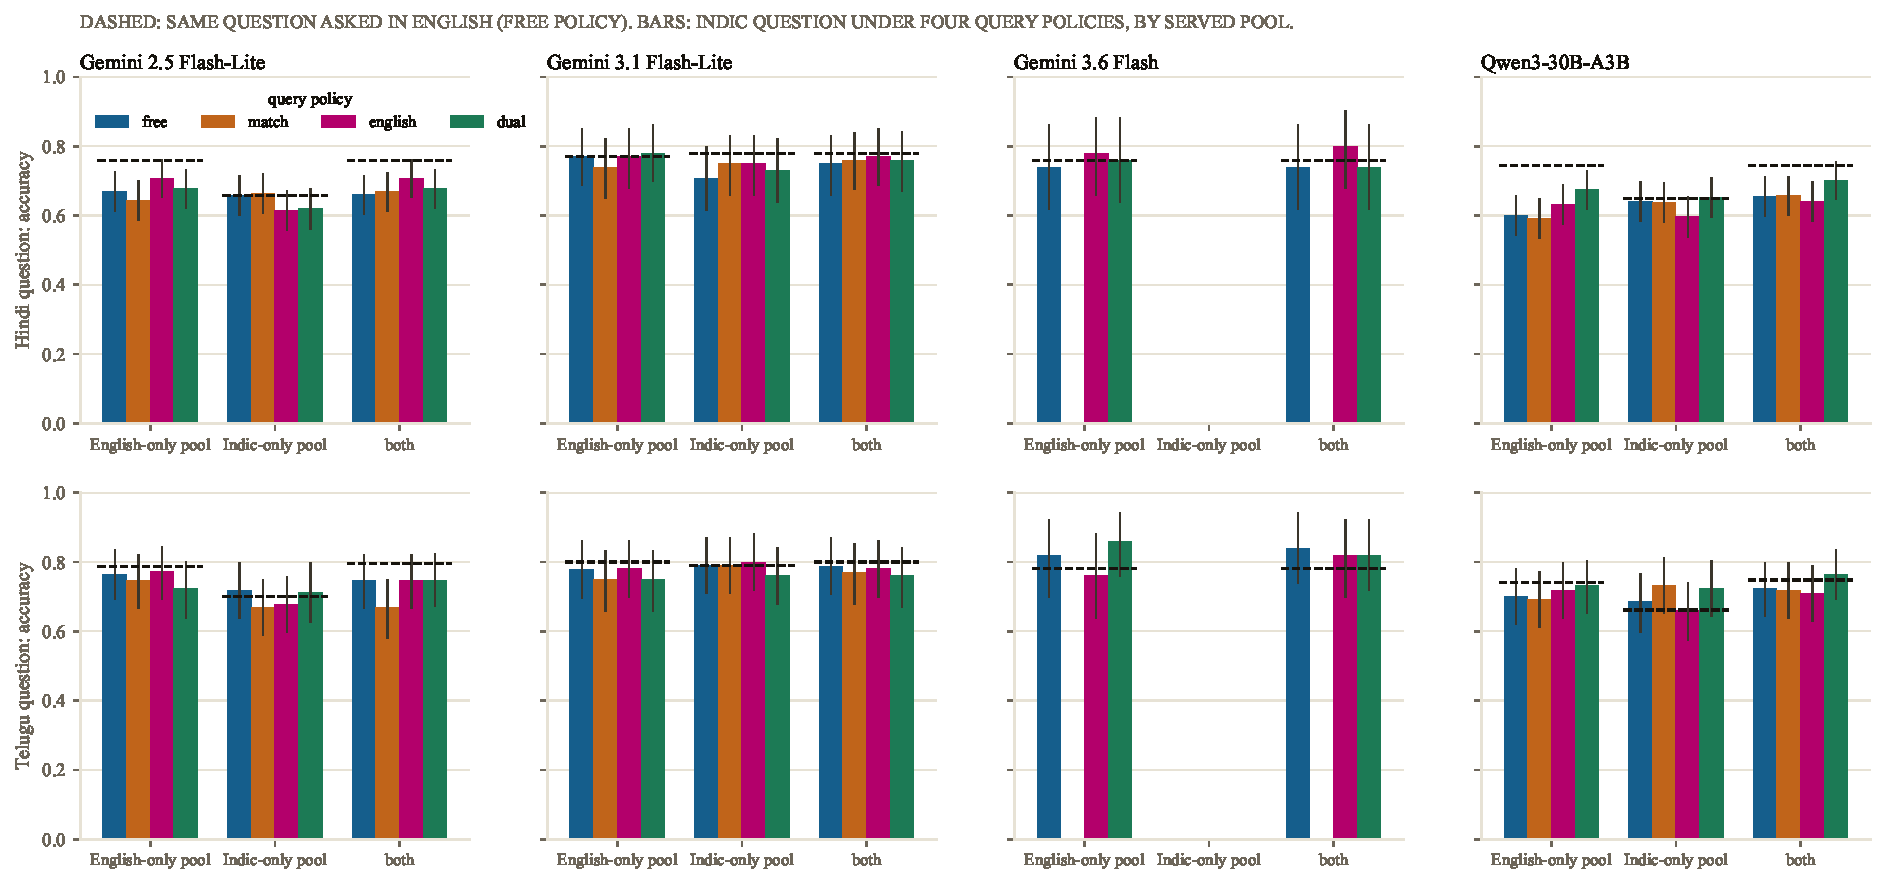
\includegraphics[width=\textwidth]{assets/fig3_policy_by_pool.pdf}
\caption{Accuracy of the Indic question under the four query policies and the three served pools, dense retriever, with item-bootstrap 95\% intervals; the dashed line is the same question asked in English under the free policy. Top row Hindi, bottom row Telugu.}\label{fig:fig3}\end{figure}
\begin{figure}[t]\centering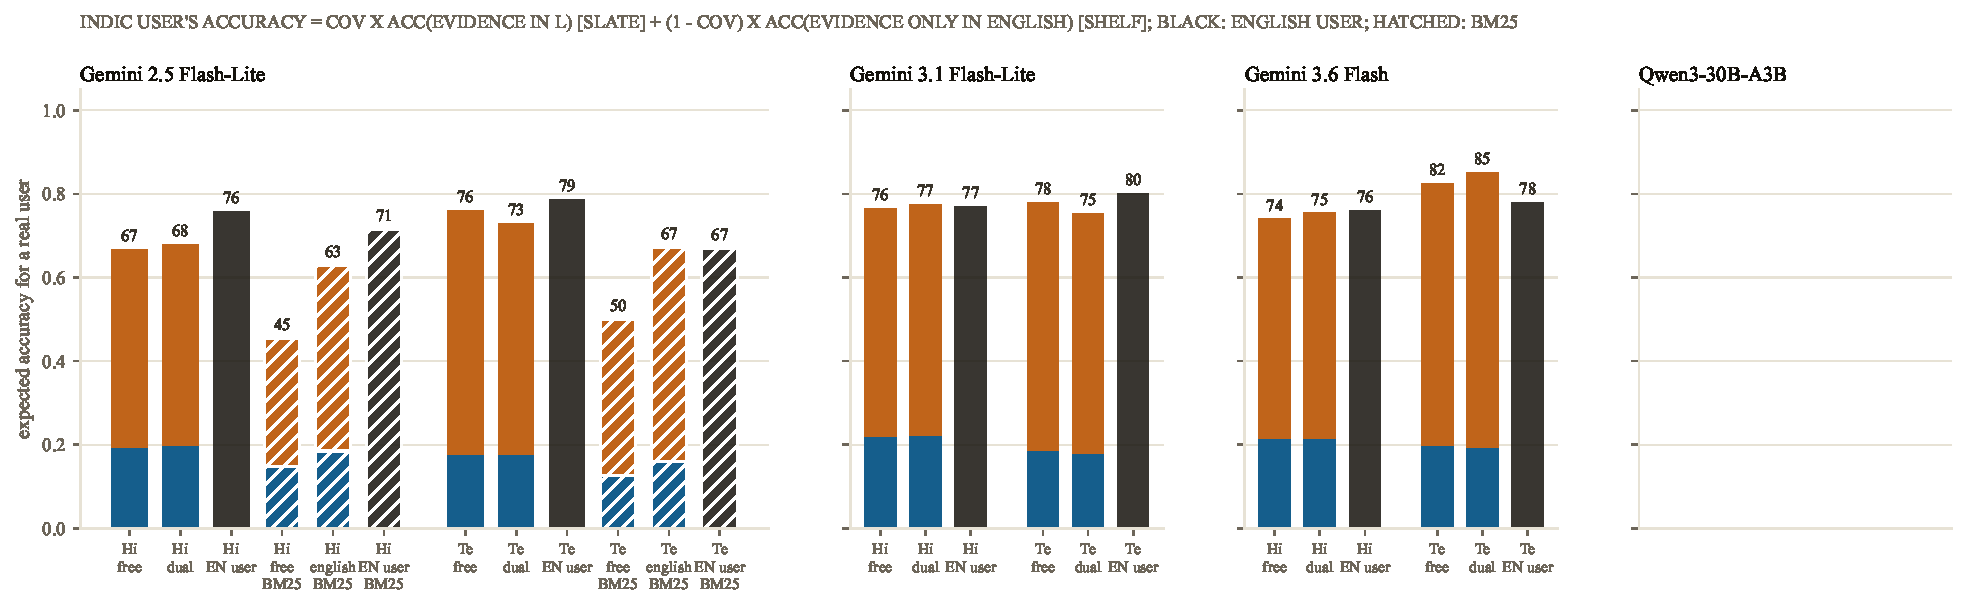
\includegraphics[width=\textwidth]{assets/fig4_decomposition.pdf}
\caption{Expected accuracy of a real Indic user from Eq.~\ref{eq:decomp}: the slate part is the share of facts the Indic Wikipedia holds times the accuracy with evidence in both languages, the orange part the share only English holds times the accuracy on the English-only pool; black is the English user. Hatched bars use BM25 instead of the dense retriever.}\label{fig:fig4}\end{figure}
\begin{figure}[t]\centering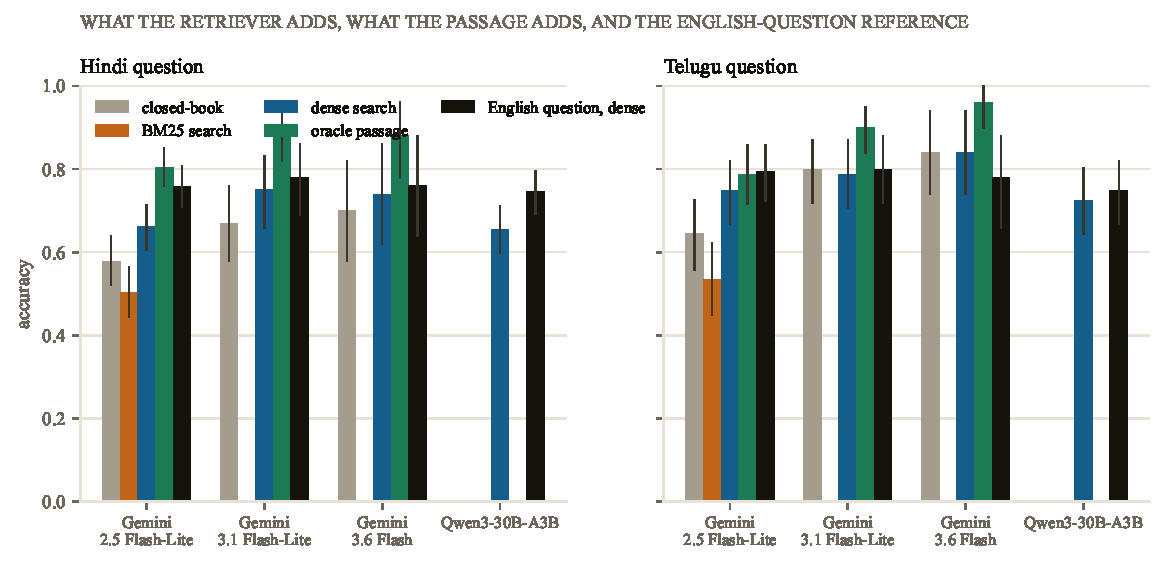
\includegraphics[width=\textwidth]{assets/fig5_retriever_oracle.pdf}
\caption{Indic question, free policy, both pools: closed-book, BM25 search, dense search, the gold passage in the prompt, and the English question with dense search, per model.}\label{fig:fig5}\end{figure}
\begin{table}[t]\centering\scriptsize
\resizebox{\textwidth}{!}{
\begin{tabular}{p{5.6cm}llllllll}
\toprule
Contrast (percentage points) & \multicolumn{2}{c}{Gemini 2.5 Flash-Lite} & \multicolumn{2}{c}{Gemini 3.1 Flash-Lite} & \multicolumn{2}{c}{Gemini 3.6 Flash} & \multicolumn{2}{c}{Qwen3-30B-A3B} \\
 & Hindi & Telugu & Hindi & Telugu & Hindi & Telugu & Hindi & Telugu \\
\midrule
Total gap: English minus Indic question (free, both pools) & \textbf{+9.4 [+4.5, +14.3]$^{*}$} & +4.7 [-1.6, +11.0] & +3.0 [-2.0, +8.0] & +1.0 [-5.1, +7.1] & +2.0 [-4.0, +10.0] & -6.0 [-14.0, +0.0] & \textbf{+9.1 [+3.8, +14.6]$^{*}$} & +2.4 [-4.7, +9.4] \\
Recovered by dual-language queries & +1.8 [-3.2, +6.8] & -2.5 [-9.2, +4.2] & +1.0 [-4.0, +6.0] & -3.0 [-10.1, +3.0] & +0.0 [-6.0, +6.0] & -2.0 [-8.0, +4.0] & +4.5 [+0.7, +8.4]$^{*}$ & +3.9 [-0.8, +9.4] \\
Recovered by English-only queries & +4.5 [+0.0, +9.1] & +0.0 [-6.3, +6.3] & +2.0 [-3.0, +7.0] & -1.0 [-6.1, +4.0] & +6.0 [+0.0, +14.0] & -2.0 [-10.0, +6.0] & -1.4 [-6.3, +3.5] & -1.6 [-7.1, +3.9] \\
Recovered by matched-language queries & +0.7 [-3.5, +4.9] & -7.9 [-14.2, -1.6]$^{*}$ & +1.0 [-3.0, +5.1] & -2.0 [-6.1, +2.0] & -- & -- & +0.3 [-2.8, +3.5] & -0.8 [-6.3, +4.7] \\
Evidence-side: both pools minus English-only pool & -0.7 [-5.2, +4.2] & -1.6 [-7.9, +4.7] & -2.0 [-7.0, +3.0] & +1.0 [-3.0, +5.1] & +0.0 [-6.0, +6.0] & +2.0 [-6.0, +10.0] & -- & -- \\
Evidence-side: both pools minus Indic-only pool & +0.3 [-3.5, +4.2] & +3.1 [-2.4, +8.7] & +4.0 [-2.0, +10.1] & +0.0 [-6.1, +6.1] & -- & -- & +1.4 [-1.8, +4.9] & +4.2 [-2.5, +11.9] \\
English queries minus matched queries, English-only pool & +6.3 [+1.7, +11.2]$^{*}$ & +2.4 [-3.1, +7.9] & +3.0 [-2.0, +8.0] & +3.0 [-2.0, +8.0] & -- & -- & -- & -- \\
English queries minus matched queries, Indic-only pool & -4.9 [-10.1, +0.7] & +0.8 [-7.1, +8.7] & +0.0 [-5.0, +5.0] & +1.0 [+0.0, +3.0] & -- & -- & -4.2 [-8.4, +0.0] & -9.4 [-18.8, -1.0] \\
Symmetric monolingual: en/en minus L/L & \textbf{+10.1 [+4.5, +15.7]$^{*}$} & +12.6 [+3.9, +21.3]$^{*}$ & -- & -- & -- & -- & -- & -- \\
Integration gap: oracle passage, English minus Indic question & \textbf{+6.3 [+2.8, +9.8]$^{*}$} & +6.3 [+0.0, +12.6] & -2.0 [-6.0, +2.0] & -1.0 [-5.0, +2.0] & -2.0 [-10.0, +4.0] & -2.0 [-6.0, +0.0] & -- & -- \\
Closed-book gap & +3.1 [-1.0, +7.3] & +3.9 [-2.4, +10.2] & +3.0 [-4.0, +10.0] & -1.0 [-7.0, +5.0] & +2.0 [-4.0, +10.0] & +0.0 [-6.0, +6.0] & -- & -- \\
Total gap under BM25 & \textbf{+18.9 [+12.9, +24.8]$^{*}$} & +11.0 [+2.4, +19.7]$^{*}$ & -- & -- & -- & -- & -- & -- \\
Symmetric monolingual under BM25 & \textbf{+35.3 [+28.7, +41.6]$^{*}$} & \textbf{+31.0 [+19.8, +42.1]$^{*}$} & -- & -- & -- & -- & -- & -- \\
Recovered by dual queries under BM25 & \textbf{+9.3 [+3.9, +14.6]$^{*}$} & +7.6 [-1.7, +16.8] & -- & -- & -- & -- & -- & -- \\
Indic question: BM25 minus dense (free, both) & \textbf{-15.7 [-21.3, -10.1]$^{*}$} & \textbf{-21.3 [-30.7, -12.6]$^{*}$} & -- & -- & -- & -- & -- & -- \\
\midrule
Policy $\times$ evidence interaction & \textbf{+11.2 [+4.2, +18.2]$^{*}$} & +1.6 [-7.9, +11.0] & +3.0 [-4.0, +10.0] & +2.0 [-3.0, +8.0] & -- & -- & -- & -- \\
\bottomrule
\end{tabular}}
\caption{Paired within-item contrasts (percentage points) with item-bootstrap 95\% intervals. $^{*}$: sign-flip permutation $p<0.05$. Bold: survives Benjamini--Hochberg over the full family of 106 tests (threshold $p \le 0.0052$). Positive total gap = the English question is answered more often. Dense retriever unless marked BM25.}
\label{tab:main}
\end{table}
\begin{table}[t]\centering\small
\resizebox{\textwidth}{!}{
\begin{tabular}{llrrrrr}
\toprule
Model & Language & Cov$_L$ & Indic user, free & Indic user, dual & Indic user, english & English user \\
\midrule
Gemini 2.5 Flash-Lite & Hindi & 29.1\% & 66.7 & 67.9 & 70.7 & 75.8 \\
\quad measured on the uncovered items & Hindi & 29.1\% & 51.4 & 50.4 & -- & 60.5 \\
\quad under BM25 & Hindi & 29.1\% & 45.4 & 58.4 & 62.9 & 71.4 \\
Gemini 2.5 Flash-Lite & Telugu & 23.6\% & 76.0 & 72.9 & 76.6 & 78.7 \\
\quad measured on the uncovered items & Telugu & 23.6\% & 56.8 & 52.7 & -- & 60.1 \\
\quad under BM25 & Telugu & 23.6\% & 49.9 & 55.9 & 67.1 & 66.9 \\
Gemini 3.1 Flash-Lite & Hindi & 29.1\% & 76.4 & 77.4 & 77.0 & 77.0 \\
Gemini 3.1 Flash-Lite & Telugu & 23.6\% & 78.0 & 75.2 & 78.0 & 80.0 \\
Gemini 3.6 Flash & Hindi & 29.1\% & 74.0 & 75.4 & 78.6 & 76.0 \\
Gemini 3.6 Flash & Telugu & 23.6\% & 82.5 & 85.1 & 77.4 & 78.0 \\
Qwen3-30B-A3B & Hindi & 29.1\% & 61.6 & 68.3 & 63.4 & 74.6 \\
\quad under BM25 & Hindi & 29.1\% & 43.3 & 59.9 & -- & 69.7 \\
Qwen3-30B-A3B & Telugu & 23.6\% & 70.6 & 74.0 & 71.5 & 74.0 \\
\quad under BM25 & Telugu & 23.6\% & 56.6 & 64.8 & -- & 68.5 \\
\bottomrule
\end{tabular}}
\caption{Expected accuracy for a real user, Eq.~\ref{eq:decomp}: Cov$_L$ is the share of the 539 XorQA questions whose Hindi or Telugu Wikipedia article verifiably states the answer; the Indic user's accuracy weights the both-pools cell by Cov$_L$ and the English-only cell by $1-$Cov$_L$; the English user is the English question on the English-only pool. `Measured' rows replace the extrapolated uncovered term by the direct run on the uncovered items (Section~\ref{sec:results-decomp}).}
\label{tab:decomp}
\end{table}

\section{Related work}
\label{sec:related}

\paragraph{Agentic search beyond English.} Monolingual browsing benchmarks exist for Chinese \citep{a2504_19314}, Korean \citep{a2606_02404,a2606_27595}, and thirteen natively authored languages without an Indic one \citep{a2610_03574}; BrowseComp-Plus fixed the corpus so that retrievers can be swapped \citep{a2508_06600}, and XBCP translated that corpus into twelve languages and measured deep-research agents with oracle retrieval, finding retrieval rather than integration to be the larger loss \citep{a2606_15345}. Multilingual GAIA variants place Hindi among the weakest languages at every model size \citep{a2505_15935,a2608_08775} and warn that part of the measured gap is translation artefact \citep{a2604_24929}. English-only taxonomies split agent failures into retrieval and utilisation \citep{a2608_01913,a2608_05212,a2609_08094}; logging what agents send to search engines is rare and English-centred \citep{a2609_19244}, and non-English queries receive fewer citations \citep{a2609_00319}. The MAST shared task evaluates Indic queries over an English corpus \citep{mast2026}; MarathiWeb evaluates two web-search models on native Marathi needs \citep{kale2026marathiweb}. None logs or forces an agent's query language for an Indic user, and none varies where the evidence lives.

\paragraph{Language preference in multilingual retrieval.} Retrievers and generators favour high-resource and query-language passages \citep{a2502_11175,a2604_20199,a2605_07249,a2509_13930}, outputs drift toward English when the evidence language mismatches \citep{a2511_09984}, and reasoning models fail to transfer knowledge across scripts \citep{a2603_17070}. DELTA showed that the measured English preference is confounded by where gold evidence exists and corrected for it statistically \citep{a2601_02956}; we manipulate it experimentally. Pipeline comparisons disagree on whether translating the query helps \citep{a2504_03616,a2510_23070,a2507_22923}, and The Cross-Lingual Cost shows the sign depends on where the documents are \citep{a2507_07543}; XRAG is the one controlled query-language ablation on a live engine, where native and translated queries were complementary \citep{a2505_10089}. CORAL lets an agent choose which-language corpus to search but reports end accuracy only \citep{a2604_25676}. Dense multilingual retrievers retrieve across languages where lexical matching cannot \citep{a2511_19324,a2402_03216}, which is why we treat the retriever as a factor. Up to half of correct cross-lingual QA answers are not attributable to any retrieved passage \citep{a2305_14332}, which is why we run a closed-book arm on every item.

\paragraph{Indic benchmarks and corpora.} Parallel Indic questions with known evidence come from IndicGenBench \citep{a2404_16816}, built on TyDi XOR \citep{a2010_11856,clark2020tydi}, MLQA \citep{a1910_07475}, and XQuAD \citep{a1910_11856}; India-centric closed-book sets include IndicQuest \citep{a2608_15535,a2504_20022}, MILU \citep{a2411_02538}, and MultiLoKo \citep{a2504_10356}. Indic retrieval resources include MIRACL \citep{a2210_09984}, IndicIRSuite \citep{a2312_09508}, IndicRAGSuite \citep{a2506_01615}, and Hindi-BEIR \citep{a2408_09437}; Health-Pariksha evaluates a fixed RAG pipeline on real Indic health queries \citep{a2410_13671}.

\paragraph{Knowledge and coverage gaps.} Factual recall in language models depends on language and script \citep{a2010_06189,a2102_00894,a2406_16135,a2510_15551}; India-centric questions are answered better in English even by strong models \citep{a2504_20022}, and code-mixing narrows the gap \citep{a2605_29637}. ECLeKTic and Where's Waldo build questions whose evidence exists in only one Wikipedia edition \citep{a2502_21228,a2610_00606}, the closed-book analogue of our evidence-side manipulation. Wikipedia's coverage asymmetry has been documented since Hecht and Gergle \citep{hecht2010tower} and runs both ways \citep{a2505_24195}; our pools keep the local Indic facts that English lacks.

\section{Limitations}
\label{sec:limits}
%% TODO(results): add the numbers referenced
Wikipedia is not the web. Our pools are complete for Hindi and Telugu but a 1.8\% sample of English Wikipedia plus the articles behind the items, so the English pool has fewer near-topic distractors than a real engine would return; the symmetric monolingual cells and the retriever factor bound, but do not remove, this asymmetry. Two languages and one Indic family of scripts each are studied; Bengali, Tamil and the others are not. The XorQA questions are human translations of English questions, so the Indic phrasing is not what a native user would type; the natively written Telugu subset is the check, not a cure. Coverage was measured by string match and two LLM reads of each article with a manual audit of 50 items; the audit found the first read too generous, which is why the second was added, and the remaining uncertainty is reported with the coverage estimate. The closed-model arm is Gemini only because a workspace guardrail on the API account blocked the other closed families during the study; the open-weight arm is one model. Models change; the model identifiers and the snapshot date are recorded. The judge is itself a Gemini model; the string rule decides most items and the audited sample bounds the rest. No live-web arm was run.

\section{Conclusion}
\label{sec:conclusion}
%% TODO
